%---------------------------------------------------------------------------
\svnidlong 
{$HeadURL: https://svn.fil.univ-lille1.fr/svn/sedoglav_PDC/trunk/Cours/08/08.tex $} 
{$LastChangedDate: 2012-11-16 17:25:48 +0100 (Fri, 16 Nov 2012) $} 
{$LastChangedRevision: 82 $} 
{$LastChangedBy: sedoglav $} 
\svnid{$Id: 08.tex 82 2012-11-16 16:25:48Z sedoglav $} 
%------------------------------------------------------------------------------
%Proposition de sujet (Fr\'ed\'eric Chyzak) donner le code d'une
%fonction recursive qui n'empile pas ses param\`etres mais qui les
%modifie \`a la vol\'ee (r\'ecursion terminale compil\'ee par
%continuation).
%------------------------------------------------------------------------------
%\begin{slide}
%  \listofslides
%  \begin{enumerate}
%  \item Notion de pile en assembleur
%    \begin{enumerate}
%    \item D\'efinition th\'eorique
%    \item Segment de pile et instructions assembleurs associ\'ees
%    \end{enumerate}
%\item[]
%  \item En~C, les variables automatiques (a.k.a.\ locales) sont stock\'ees dans la pile
%\item[]
%  \item Appel de fonction en~C (point de vue assembleur)
%    \begin{enumerate}
%    \item Les instructions assembleur \texttt{call} et \texttt{ret}
%%    \item Passage de param\`etres par la pile
%    \end{enumerate}
%%  \item D\'ebordement de pile
%  \end{enumerate}    
%\end{frame}
%------------------------------------------------------------------------------
\begin{frame}
  \section{Notion de pile en assembleur~: d\'efinitions th\'eoriques et pratiques}%
Sch\'ematiquement, une pile est  une structure de donn\'ees lin\'eaire
pour laquelle les insertions et les suppressions d'\'el\'ements se font
toutes \textit{du  m\^eme    cot\'e}.     On  parle    de    structure
LIFO~: Last In First Out.
\par
Plus formellement, on peut consid\'erer un ensemble d'\'el\'ements~$E$
et  noter~$\mathrm{Pil}(E)$ l'ensemble de  toutes  les piles sur~$E$.  
Par  exemple, les entiers peuvent  constituer l'ensemble~$E$~; la pile
vide~$P_{0}$    est dans~$\mathrm{Pil}(E)$.  Les op\'erations usuelles
sur une pile sont~:
\begin{itemize}
\item $\mathrm{estVide}$   est   une application  de~$\mathrm{Pil}(E)$
  dans~${(\mathrm{vrai},\mathrm{faux})}$,~${\mathrm{estVide}(P)}$  est
  vrai si, et seulement si,~$P$ est la pile~$P_{0}$.
\item       $\mathrm{empiler}$         est         une     application
  de~${E\times\mathrm{Pil}(E)}$ dans~${\mathrm{Pil}(E)}$.
\item          $\mathrm{depiler}$          est  une       application
  de~${\mathrm{Pil}(E)\setminus P_{0}}$ dans~$\mathrm{E}$.
\item       $\mathrm{supprimer}$        est    une         application
  de~${\mathrm{Pil}(E)\setminus P_{0}}$ dans~$\mathrm{Pil(E)}$.
\end{itemize}
\end{frame}
%------------------------------------------------------------------------------
\begin{frame}
Si~$x$ est un  \'el\'ement de~$E$, les  relations satisfaites par une
pile~$P$ et ces op\'erations sont~:
\begin{enumerate}
\item ${\mathrm{estVide}(P_{0})=\mathrm{vrai}}$
\item ${\mathrm{supprimer}(\mathrm{empiler}(x,P))=P}$
\item ${\mathrm{estVide}(\mathrm{empiler}(x,P))=\mathrm{faux}}$
\item ${\mathrm{depiler}(\mathrm{empiler}(x,P))=x}$
\end{enumerate}
Cette derni\`ere r\`egle caract\'erise les piles.
\end{frame}
%------------------------------------------------------------------------------
\begin{frame}
  \frametitle{Implantation d'une pile (architecture Intel~$32$)}%
  Un segment de la m\'emoire est d\'evolu \`a la pile.
  
  Les registres \%SS et \%ESP sont deux registres servant \`a g\'erer la pile~:
  \begin{itemize}
  \item[\%SS] (Stack Segment i.e.\ segment de pile) est un registre~$16$
    bits contenant l'adresse du segment de pile courant~;
  \item[]
  \item[] L'assembleur vous fera manipuler une pile qui est stock\'ee ``en fond
    de panier'', c.\`a.d dans les adresses les plus hautes de la
    m\'emoire. Ainsi, la base de la pile se trouve \`a l'adresse maximale,
    et elle s'accroit vers les adresses basses. 
  \item[]
  \item[\%ESP] (Stack Pointer i.e.\ pointeur de pile) est le d\'eplacement
    pour atteindre le sommet de la pile.
  \end{itemize}
  \par\medskip 
  Ainsi, \%ESP pointe sur le dernier mot machine occup\'e de la pile en m\'emoire.
\end{frame}
%------------------------------------------------------------------------------
\begin{frame}
  \frametitle{Notion de pile en assembleur~: instructions assembleurs
    associ\'ees (Intel~$32$)}
  Les modification de la structure de la pile se font par les
  instructions~:
  \begin{itemize}
  \item\textbf{push} reg~: (empiler depuis le registre reg).  Lorsque l'on
    empile un \'el\'ement sur la pile, l'adresse contenue dans \%ESP est 
    d\'ecr\'ement\'ee de~$4$ octets (car un emplacement de la pile est un 
    mot machine de~$32$ shannons).  En effet, lorsque l'on parcourt
    la pile de la base vers le sommet, les adresses d\'ecroissent.
  \item\textbf{pop} reg~: (d\'epiler vers le registre reg). Cette
    instruction incr\'emente de~$4$ octets la valeur de \%ESP.
    Attention, lorsque la pile est vide \%ESP pointe sous la pile
    (l'emplacement m\'emoire en-dessous de la base de la pile) et un
    nouveau pop provoquera une erreur.
  \end{itemize}
  \par\medskip
  Il est aussi possible --- pour lire ou modifier des valeurs dans la
  pile --- d'utiliser les r\'ef\'erences m\'emoire~: \\
  movl \%SS:4(\%ESP),\%EAX
\end{frame}
%------------------------------------------------------------------------------
\begin{frame}
  \begin{center}
    \begin{tabular}{lc}
      \begin{minipage}[b]{3.5cm}
        \begin{itemize}
        \item RX3 est \%ESP~;
        \item \%ESP pointe sur 
        l'octet venant d'\^etre 
        empil\'e~;
        \item On empile un mot machine~($4$ octets).
        \end{itemize}
      \end{minipage}
      & 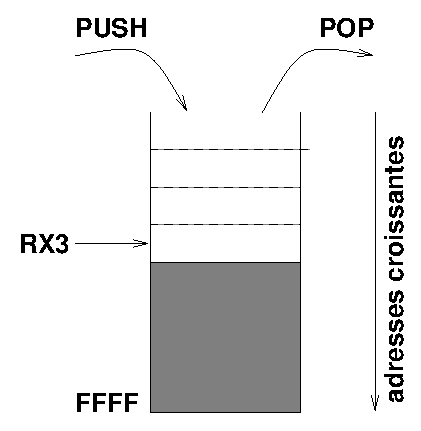
\includegraphics[scale=.8,angle=90]{pile} \\
    \end{tabular}
  \end{center}
\end{frame}
%------------------------------------------------------------------------------
\begin{frame}[fragile]
  \section{Repr\'esentation des variables automatiques}%
  Les variables \emph{automatiques} (locales \`a une fonction) sont stock\'ees dans la pile.
  \par\smallskip
  Le registre \%EBP (Base Pointer) contient un d\'eplacement
  correspondant \`a une position dans la pile.
  \par\smallskip
  Il sert \`a pointer sur une donn\'ee dans la pile. 

        Repr\'esentation d'une variable automatique dans la pile~:
\begin{verbatim}
int globale = 7 ;          .globl globale .data                 
                  globale: .long   7                   
                           .text                        
int                        .globl main .type main,@function   
main                 main:                                
(void)                      ....                         
{                           movl    %esp, %ebp           
  int locale ;              subl    $8, %esp  
  locale = 1 ;              .... 
  return 0 ;                movl    $1, -4(%ebp)         
}                           ....                         
\end{verbatim}
\end{frame}
%------------------------------------------------------------------------------
\begin{frame}[fragile]
  \frametitle{Repr\'esentation des variables automatiques}%
      \begin{tabular}{ccc}
        \verb?movl %esp, %ebp? & 
     \verb?subl $8, %esp? \\
    \begin{tabular}[b]{c|c|}
      \hline
      \%ESP & data   \\\hline
      & $4$ octets  \\\hline
      & $\vdots$   \\
      \hline
      FFFF & bas de pile \\\hline
    \end{tabular} &
    \begin{tabular}[b]{c|c|}
      \hline
      \%ESP & vide   \\\hline
      & vide   \\\hline
      \%EBP & data   \\\hline
      & $4$ octets  \\\hline
      & $\vdots$   \\
      \hline
      FFFF & bas de pile \\\hline
    \end{tabular} \\
        \%EBP mis en place &
        r\'eserver de l'espace \\
    &    \verb?movl    $1, -4(%ebp)? \\
   & \begin{tabular}[b]{c|c|}
      \hline
      \%ESP & vide   \\\hline
      & $1$        \\\hline
      \%EBP & data   \\\hline
      & $4$ octets  \\\hline
      & $\vdots$   \\
      \hline
      FFFF & bas de pile \\\hline
    \end{tabular} \\
     & affecter la variable 
  \end{tabular}
\end{frame}
%------------------------------------------------------------------------------
\begin{frame}[fragile]
  \frametitle{Repr\'esentation de variables de types diff\'erents et manipulation}%
        Peu importe le type des variables automatiques que l'on veut repr\'esenter,
        la m\'ethode est la m\^eme~:
        \par\medskip
\begin{verbatim}
int                            .text                           
main                           .globl main                    
(void)                         .type main, @function    
{                        main: ....                      
  struct Gauss{                 movl %esp, %ebp         
    int re ;                    subl $24, %esp          
    int im ;                    ....                    
  } var = {                     movl   $1, -8(%ebp)       
    .re = 1 ,                   movl   $1, -4(%ebp)       
    .im = 1 ,                   movb   $97, -10(%ebp) 
  } ;                           movb   $98, -9(%ebp)  
                                movb   -9(%ebp), %dl  
  char tab[2] = {'a','b'} ;     leal   -10(%ebp), %eax
  tab[0] += tab[1] ;            addb   %dl, (%eax)    
  return 0 ;                    ....                    
}                                    
\end{verbatim}
\end{frame}
%------------------------------------------------------------------------------
\begin{frame}
  \section{Appel de fonction en~C}
  \frametitle{Rappel sur les registres associ\'es \`a l'ex\'ecution du code}%

        Le code ex\'ecutable d'un programme se pr\'esente sous la forme 
        d'une suite finie contig\"ue d'octets stock\'ee dans un segment 
        de la m\'emoire.
        \par\medskip
        \textbf{Le registre \%\textsc{CS} (Code Segment).} Ce registre~$16$
        bits contient le num\'ero du segment m\'emoire dans lequel
        sont stock\'e les instructions assembleur du code \`a
        ex\'ecuter.  On ne peut pas acc\'eder directement \`a ce
        registre.
        \par\medskip
        \textbf{Le registre \%EIP (Instruction Pointer).}  Le
        registre \%\textsc{eip} contient l'offset de la prochaine
        instruction \`a ex\'ecuter.  Il est modifi\'e automatique \`a
        chaque ex\'ecution et peut \^etre manipul\'e par des
        instruction du type \texttt{jmp}, \texttt{call}, \texttt{ret},
        etc. On ne peut pas acc\'eder directement \`a ce registre.
\end{frame}
%------------------------------------------------------------------------------
\begin{frame}[fragile]
  \frametitle{Les instructions assembleur \texttt{call} et
  \texttt{ret}}%

        L'appel d'une \emph{routine} se fait par %
        \verb+call label_routine+. 
        Soit un code implant\'e \`a l'adresse
        1000 et une routine \`a l'adresse 1100.

\begin{verbatim}
  1000 mov $1,%eax         +---> label: 1100 shl $1,%eax    
  1002 mov $3,%ebx         |            1102 add %ebx,%eax    
  1004 CALL label  --------|            1104 and $7,%eax     
  1007 mov $2,%eax <-------|            1106 add '0',%eax   
  1009 int 0x80            |____        1108 RET          
\end{verbatim}
        
Le sous-programme doit contenir l'instruction \textsc{ret} qui permet de revenir au
programme appelant. 


Lors du \textsc{call}, \%\textsc{eip} re\c{c}oit la valeur 1100, adresse de la prochaine
instruction \`a ex\'ecuter, tandis que l'adresse de retour 1007 est
empil\'ee sur la pile.

Sur le \textsc{ret}, le sommet de pile de valeur 1007 est d\'epil\'e, et son
contenu est rang\'e dans \%\textsc{eip}.
\end{frame}
%------------------------------------------------------------------------------
\begin{frame}[fragile]
  \frametitle{Appel de fonction en~C (sans param\`etre)}%
\begin{verbatim}
                                   .text                        
int                                .globl UN                        
UN                            UN:                                
(void)                             ...                        
{                                  movl    $1, %eax        
  return 1 ;                       ...                        
}                                  ret                       
          
                                  .globl main                        
int                         main:                                
main                                ...                        
(void)                             movl    %esp, %ebp        
{                                  subl    $8, %esp        
  int var ;                        ....                        
  var = UN() ;                     call    UN                
  return 0 ;                       movl    %eax, -4(%ebp)        
}                                  movl    $0, %eax        
/* Remarquez que la valeur         ...                        
   de retour transite par          ret                        
   le registre %eax        */      ...                     
\end{verbatim}
\end{frame}
%------------------------------------------------------------------------------
\begin{frame}
  \frametitle{Ce qui se passe sur la pile}%
  \begin{center}
      \begin{tabular}{cccc}
     \begin{tabular}[b]{c|c|}
      \hline
      \%ESP & vide   \\\hline
      & var.\ aut.\ \\\hline
      \%EBP & data   \\\hline
      & $4$ octets  \\
      \hline
      FFFF & bas de pile \\\hline
    \end{tabular} & $\rightarrow$
     \begin{tabular}[b]{c|c|}
      \hline
      \%ESP & adresse  \\
 & de retour   \\\hline
          & vide   \\\hline
      & var.\ aut.\ \\\hline
      \%EBP & data   \\\hline
      & $4$ octets  \\
      \hline
      FFFF & bas de pile \\\hline
    \end{tabular} 
         \\ 
         avant le call & pendant le call \\
         & $\downarrow$ \\
         &
     \begin{tabular}[b]{c|c|}
      \hline
      \%ESP & vide   \\\hline
      & var.\ aut.\ \\\hline
      \%EBP & data   \\\hline
      & $4$ octets  \\
      \hline
      FFFF & bas de pile \\\hline
    \end{tabular} \\
         
         & apr\`es le ret 
  \end{tabular}
  \end{center}
\end{frame}
%------------------------------------------------------------------------------
\begin{frame}
  \section{Passage de param\`etres par la pile}%
        Comme toutes variables automatiques, les param\`etres sont stock\'es
        dans la pile. Dans une fonction~C les variables et 
        les param\`etres sont g\'er\'es en suivant les \'etapes~:
        \begin{enumerate}
        \item Sauver le pointeur de base de pile courant sur la pile~;
        \item Se donner un nouveau pointeur de base de pile~;
        \item D\'eclarer les variables automatiques sur la pile~;
        \item[] En cas d'appel de fonction avec passage de param\`etres~:
        \item Empiler les param\`etres sur la pile~;
        \item Effectuer un \texttt{call} (qui empile automatiquement
        l'adresse de retour sur la pile)~;
        \item[] Dans la fonction appel\'ee, on peut utiliser l'espace
        de pile associ\'ee aux param\`etres~;
         Cette fonction se termine par un \texttt{ret} (qui  
        d\'epile automatiquement l'adresse de retour)~;
        \item Suprimer l'espace de pile --- maintenant inutile --- 
        associ\'e aux param\`etres.
        \end{enumerate}
        \end{frame}
%------------------------------------------------------------------------------
\begin{frame}[fragile]

\begin{verbatim}
int                       .text 
PlusUn                    .globl PlusUn 
(int par)          PlusUn:                                
{                          pushl   %ebp                
  return par+1 ;           movl    %esp, %ebp        
}                          movl    8(%ebp), %eax        
                           incl    %eax                
                           leave ret                        
                           .globl main                        
                     main:                                
                           pushl   %ebp                
int                        movl    %esp, %ebp        
main                       subl    $8, %esp        
(void)                     movl    $7, -4(%ebp)        
{                          subl    $12, %esp        
  int var ;                pushl   -4(%ebp)        
  var = 7 ;                call    PlusUn                
  return PlusUn(var) ;     addl    $16, %esp        
}                          leave
                           ret                     
\end{verbatim}
\end{frame}
%------------------------------------------------------------------------------
\begin{frame}
  \frametitle{Ce qui se passe sur la pile}%
  \begin{center}
    \begin{tabular}{cc}
      \begin{tabular}[b]{c|c|}
        \hline
        \%ESP & adresse  \\
        & de retour   \\\hline
        & $4$ octets  \\
        \hline
        FFFF & bas de pile \\\hline
      \end{tabular} &
      \begin{tabular}[b]{c|c|}
        \hline
        \%ESP & \%EBP\_old   \\\hline
        & adresse  \\
        & de retour   \\\hline
        & $4$ octets  \\
        \hline
        FFFF & bas de pile \\\hline
      \end{tabular}       \\
      d\'ebut de fonction & empilement de l'ancien \\
      & pointeur de base  \\
    \end{tabular}
  \end{center}
\end{frame}
%------------------------------------------------------------------------------
\begin{frame}
  \frametitle{Ce qui se passe sur la pile}%
  \begin{center}
    \begin{tabular}{cc}
      \begin{tabular}[b]{c|c|}
        \hline
        \%ESP   & \\
        $\downarrow$     & \%EBP\_old   \\
        \%EBP1 & \\
        \hline
        & adresse  \\
        & de retour   \\\hline
        & $4$ octets  \\
        \hline
        FFFF & bas de pile \\\hline
      \end{tabular} &
      \begin{tabular}[b]{c|c|}
        \hline
        \%ESP &    \\\hline
        & var.\ loc.\   \\\hline
        \%EBP1 & \%EBP\_old   \\\hline
        & adresse  \\
        & de retour   \\\hline
        & $4$ octets  \\
        \hline
        FFFF & bas de pile \\\hline
      \end{tabular} 
      \\
      placement du nouveau & cr\'eation de variables \\
      pointeur de base &      automatiques 
    \end{tabular}
  \end{center}
\end{frame}
%------------------------------------------------------------------------------
\begin{frame}
  \begin{center}
    \begin{tabular}{cc}
      \begin{tabular}[b]{c|c|}
        \hline
        \%ESP & param\`etres    \\\hline
        & var.\ loc.\   \\\hline
        \%EBP1 & \%EBP\_old   \\\hline
        & adresse  \\
        & de retour   \\\hline
        & $4$ octets  \\
        \hline
        FFFF & bas de pile \\\hline
      \end{tabular} &
      \begin{tabular}[b]{c|c|}
        \hline
        \%ESP       & adresse  \\
        & de retour   \\\hline
        & param\`etres    \\\hline
        & var.\ loc.\   \\\hline
        \%EBP1 & \%EBP\_old   \\\hline
        & adresse  \\
        & de retour   \\\hline
        & $4$ octets  \\
        \hline
        FFFF & bas de pile \\\hline
      \end{tabular} 
      \\
      empilement de param\`etres & 
      apr\`es un \texttt{call} \\

    \end{tabular}
  \end{center}
\end{frame}
%------------------------------------------------------------------------------
\begin{frame}[fragile]
  \begin{center}
    \begin{tabular}{ccc}
      \begin{tabular}[t]{c|c|}
        \multicolumn{2}{c}{Pile (fonction appell\'ee)} \\
        \hline
        \%ESP & var.\ loc.\   \\\hline
        \%EBP & \%EBP1   \\\hline
        & adresse  \\
        & de retour   \\\hline
        & param\`etres    \\\hline
        & var.\ loc.\   \\\hline
        \%EBP & \%EBP\_old   \\\hline
        & adresse  \\
        & de retour   \\\hline
        & $\vdots$\\
      \end{tabular} &
      \begin{minipage}[t]{5cm}
        \`A la fin de la fonction appell\'ee
        \par
        1) une instruction \texttt{leave} permet d'enlever de la
          pile l'espace associ\'e aux variables automatiques et au stockage
          du pointeur de base. De plus, elle r\'eaffecte au registre
          \%EBP la valeur du pointeur de base de la fonction appelante.
      \end{minipage} \\[\medskipamount]
      \begin{minipage}[t]{4cm}
        2) l'instruction \texttt{ret} d\'epile l'adresse de retour et
          positionne le registre pointeur d'instruction \`a cette adresse.
      \end{minipage} &
      \begin{minipage}[t]{5cm}
        3) il ne reste plus qu'\`a supprimer de la pile l'espace
        associ\'e aux param\`etres (\verb?addl $16,%esp?)
        pour se retrouver dans la situation d'avant l'appel de
        fonction.
      \end{minipage}
    \end{tabular}
  \end{center}
\end{frame}
%------------------------------------------------------------------------------
\begin{frame}[fragile]
  \section{Passage de param\`etre~: une copie est faite sur la pile}%
  \frametitle{Exemple incorrect de permutation}
\begin{verbatim}
                                    .text                    
                                    .globl PER           
void                         PER:                    
PER                                  pushl %ebp          
(int alpha, int beta)                movl  %esp, %ebp        
{                                    subl  $4, %esp       
   int tmp ;                         movl  8(%ebp), %eax     
   tmp = alpha ;                     movl  %eax, -4(%ebp)
   alpha = beta ;                    movl  12(%ebp), %eax
   beta = tmp;                       movl  %eax, 8(%ebp) 
   return ;                          movl  -4(%ebp), %eax 
}                                    movl  %eax, 12(%ebp)
                                     leave               
                                     ret                 
\end{verbatim}
\end{frame}
%------------------------------------------------------------------------------
\begin{frame}[fragile]
\begin{verbatim}
int                            .globl main   
main                      main:         
(void)                         pushl %ebp     
{                              movl  %esp, %ebp    
   int a = 1 ;                 subl  $8, %esp  
   int b = 2 ;                 andl  $-16, %esp    
   PER(a,b) ;                  movl  $1, -4(%ebp)  
   return 0 ;                  movl  $2, -8(%ebp)  
}                              subl  $8, %esp  
                               pushl -8(%ebp)  
/* certains compilateurs       pushl -4(%ebp)  
placent variables              call  PER       
automatiques et param\`etres   addl  $16, %esp 
aux m\^emes endroits           movl  $0, %eax  
(pas de push) */               leave           
                               ret            
\end{verbatim}
\end{frame}
%------------------------------------------------------------------------------
\begin{frame}[fragile]
  \frametitle{Passage de param\`etre par adresse~: les adresses sont copi\'ees sur la pile}%
\begin{verbatim}
                                  .text         
                                  .globl PER                   
                           PER:                     
void                              pushl %ebp             
PER                               movl  %esp, %ebp     
(int *alpha, int *beta)           subl  $24, %esp      
{                                 movl  8(%ebp), %eax  
  int tmp ;                       movl  (%eax), %eax     
  tmp = *alpha ;                  movl  %eax, -12(%ebp)   
  *alpha = *beta ;                movl  12(%ebp), %eax 
  *beta = tmp ;                   movl  (%eax), %edx
  return ;                        movl  8(%ebp), %eax 
}                                 movl  %edx, (%eax)  
                                  movl  12(%ebp), %edx   
                                  movl  -12(%ebp), %eax   
                                  movl  %eax, (%edx)  
                                  leave                           
                                  ret                 
\end{verbatim}
\end{frame}
%------------------------------------------------------------------------------
\begin{frame}[fragile]
  \frametitle{La fonction appelante}%
\begin{verbatim}
                           .globl main                
                    main:                        
                           pushl %ebp                
                           movl  %esp, %ebp        
                           subl  $8, %esp        
                           andl  $-16, %esp        
int                        movl  $1, -4(%ebp)        
main                       movl  $2, -8(%ebp)        
(void)                     subl  $8, %esp        
{                          leal  -8(%ebp), %eax  
   int a  ;                pushl %eax                
   int b ;                 leal  -4(%ebp), %eax  
   a = 1 ;                 pushl %eax                
   b = 2 ;                 call  PER                
                           addl  $16, %esp        
   PER(&a,&b) ;            movl  $0, %eax        
   return 0;               leave                              
}                          ret              
\end{verbatim}
\end{frame}
\end{document}
%------------------------------------------------------------------------------
\begin{frame}
  \section{Passage de param\`etre de type structure}%
\begin{verbatim}
typedef  struct Gauss_t{              .text                      .globl main   
    int re ;                    .globl UN               main:             
    int im ;                UN:                              pushl   %ebp    
  } Gauss_t ;                   pushl %ebp                   movl  %esp, %ebp  
                                movl  %esp, %ebp             subl  $8, %esp    
void UN(Gauss_t par){           subl  $8, %esp               andl  $-16, %esp  
   par.re = 2 ;                 movl  8(%ebp), %eax          movl  $1,-8(%ebp) 
}                               movl  12(%ebp), %edx         movl  $1,-4(%ebp) 
                                movl  %eax, -8(%ebp)         subl  $8, %esp   
int main(void){                 movl  %edx, -4(%ebp)         pushl -4(%ebp)    
                                movl  $2, -8(%ebp)           pushl -8(%ebp)    
   struct Gauss_t var ;         leave                        call  UN      
   var.re = 1 ;                 ret                          addl  $16,
   var.im = 1 ;                                              movl  $0, %eax   
                                                             leave         
   UN(var) ;                                                 ret             

   return 0 ;
}                         
\end{verbatim}
\end{frame}
%------------------------------------------------------------------------------
\begin{frame}
  \frametitle{Passage de param\`etre de type structure avec structure retourn\'ee}%
\begin{verbatim}
typedef  struct Gauss_t{                   .text                 
    int re ;                          .globl UN                      .globl main   
    int im ;                     UN:                          main:           
  } Gauss_t ;                       pushl %ebp               pushl %ebp            
                                    movl  %esp, %ebp         movl  %esp, %ebp  
struct Gauss_t UN(Gauss_t par){     subl  $8, %esp           subl  $24, %esp   
   par.re = 2 ;                     movl  8(%ebp), %eax      andl  $-16, %esp  
   return par ;                     movl  12(%ebp), %edx     movl  $1, -8(%ebp)
}                                   movl  16(%ebp), %ecx     movl  $1, -4(%ebp)
                                    movl  %edx, -8(%ebp)     leal  -16(%ebp),%eax       
int main(void){                     movl  %ecx, -4(%ebp)     subl  $4, %esp    
                                    movl  $2, -8(%ebp)       pushl -4(%ebp)    
   struct Gauss_t var,res ;         movl  -8(%ebp), %edx     pushl -8(%ebp)    
   var.re = 1 ;                     movl  -4(%ebp), %ecx     pushl %eax               
   var.im = 1 ;                     movl  %edx, (%eax)       call  UN                                            
                                    movl  %ecx, 4(%eax)      addl  $12, %esp   
   res = UN(var) ;                  leave                    movl -16(%ebp),%eax
   var.im = res.re ;                ret   $4                 movl %eax,-4(%ebp)
   return 0 ;                                                movl  $0,%eax
}                                                            leave ret
 \end{verbatim}
\end{frame}
%------------------------------------------------------------------------------

%------------------------------------------------------------------------------
% Modele
%------------------------------------------------------------------------------
\begin{frame}
  \section{}%
\end{frame}
%------------------------------------------------------------------------------
